\section{Implementation}
This section describes how the developed program with the components described earlier, would behave in the web. To ensure that the program does not harm the tested forum when it behaves incorrectly, a web forum is set up locally and a complete work cycle is tested on this particular forum.

\subsection{Implementation environment}
The test-forum must have access to a database source. It contains for the duration of the tests 50,000 entries. These entries include a post title, post content and a unique web URL that is used as ID. The articles are stored in a NoSQL database `Elasticsearch`. It has the advantage that with only one search request to the database, the first 20 posts that match the search term can be returned easily.\\ The test forum is created locally in order to avoid a large number of requests to a forum available on the internet. A thorough evaluation could harm the internet forum caused by too much network.\\
All programs are written in `JavaScript`. The forum will run on a `Node.js Server`.

\subsubsection{Structure of the forum}
The structure of the test-forum should be has close as possible to an original internet forum. At the same time it should be easy to change web pages for registration, signup and search. This allows fast debugging when the program extracts incorrect information for registration, login or search.
The test-forum includes a login , a registration and a search page to which is redirected to after a successful login.

\subsubsection {Registration in a forum}
The most common registration form that can be found in various internet forums, consists of 2 fields for the password, 2 fields for the email, a field for the user name and a checkbox that the forum terms are accepted. This is demonstrated by the following code sample.

\begin{figure}[h!]
\begin{lstlisting}[language=HTML5]
<form action="/reg" method="post">
Nutzername: <input type="text" name="fname"></br>
Email: <input type="text" name="email"></br>
Validate Email: 
<input type="text" name="re_email"></br>
Password: <input type="password" name="pwd"></br>
Validate Password: 
<input type="password" name="re_pwd"></br>
Accept AGB:<input type="checkbox" name="AGB"></br>
<input type="hidden" name="val1" value="val1">
<input type="hidden" name="val2" value="val2">
<input type="submit" value="Submit">
</form>
\end{lstlisting}
\caption{HTML-Code f�r die Erstellung einer Registrierungsseite mit Nutzernamen, Email- und Passwordfeldern sowie Checkbox}
\end{figure}

From figure 2 it is easy to evaluate whether the registration process will be successful.
Expected would be a `POST Request` to the top-level domain + form action with the POST parameters `fname`, `email`, `re\_email`, `pwd`,\\ `re\_pwd`, `AGB`, as well as hidden key-value pairs, `val1 = hiddenvalue1` and `val2 = hiddenvalue2`.\\
The fields `fname`, `email` and `pwd` should be filled with username, email and password and confirmed in the fields `re\_email` and `re\_pwd` by repeating.\\
If the HTTP server is started , the registration page is analyzed and the following request sent to the server :

\begin{figure}[ht]
\begin{lstlisting}[language=HTML5]
http://localhost:12345/reg
{ val2: 'hiddenvalue2',
val1: 'hiddenvalue1',
AGB: 'on',
re_pwd: 'AjZt198#ev',
pwd: 'AjZt198#ev',
re_email: 'jpm96353@adiaq.com',
email: 'jpm96353@adiaq.com',
fname: 'Dominik' }
verification email to : jpm96353@adiaq.com
\end{lstlisting}
\caption{Inhalt des POST-Requests, den das Programm an das Forum bei einem Registrierungsaufruf sendet}
\end{figure}

It should be noted that the program has created an own email. It comes from the website ` `10minutemail`~\footnote{https://10minutemail.net/ visited: 10.06.2015}. This internet site provides a free e-mail address, where e-mails can be received and sent with for 10 minutes. The registration request has been sent to the correct URL of the server, which is shown by the `http://localhost:12345/reg`. Furthermore, all the necessary parameters of the POST requests and also the repetition of the fields email and password have been filled in correctly. The checkbox for the GTC is ticked and also all the hidden input fields in the form were transmitted. Overall, this is a valid registration request, which is acknowledged by the forum with a validation email to the specified email address.

he program checks every 5 seconds if the email has been received (Figure 4). Should this be the case, the email content is analyzed and every found link called. If there is no new e-mail within 10 minutes, the registration attempt is considered as failed and communicated to the user, because the email address is valid for 10 minutes only.

\begin{figure}[ht]
\begin{lstlisting}[language=HTML5]
registered
No new emails
No new emails
No new emails
location='readmail.html?mid=KfKcm0'
https://10minutemail.net/readmail.html?mid=KfKcm0
clicked: http://localhost:12345/validateUser?user=jpm96353@adiaq.com
\end{lstlisting}
\caption{Das Programm wartet auf Registrierungs-Email und ruft alle Links in der Email auf.}
\end{figure}

The validation link that the forum has generated and sent in the email is invoked (Figure 4) and the validation test will be sent to the forum, which markes the user as an active user (Figure 5).

\begin{figure}[ht]
\begin{lstlisting}[language=HTML5]
/validateUser?user=jpm96353@adiaq.com
validate:
jpm96353@adiaq.com
\end{lstlisting}
\caption{Das Forum validiert den Nutzeraccount, da der Validierungslink best�tigt wurde.}
\end{figure}

If the registration process fails, the registration form can be recreated and changes can be made to the field evaluation metrics. A new retesting can be done without burdening web forums. There is the option for the program to skip the registration step. If the user has already created a user account manually , he can pass the account information to the program through input parameters. Rather than registering, it now uses the existing user account. Thus, if the technical program registration failed, it is still possible to crawl the forum automatically.

\subsubsection {Forum login}
If account details are given when the program starts, they should also be used for the login. Otherwise account details from the registration step are used. The login request should include three parameters, once the user name, once the password, and once a checkbox. The checkbox specifies whether you want to stay logged in on the site in order to not reenter the user data on a next visit. These are the most common login forms that exist on the internet (Figure 6).

\begin{figure}[ht]
\begin{lstlisting}[language=HTML5]
<form action="/log" method="post">
Nutzername: 
<input type="text" name="fname"></br>
Password: 
<input type="password" name="pwd"></br>
Eingeloggt bleiben: 
<input type="checkbox" name="remember">
<input type="submit" value="Submit">
</form>
\end{lstlisting}
\caption{HTML-Code, der die Loginseite des Forums darstellt}
\end{figure}


\begin{figure}[h!]
\begin{lstlisting}[language=HTML5]
loginattempt: 
{fname:'Dominik',
remember: 'on',
pwd:'AjZt198#ev'}
\end{lstlisting}
\caption{Eingehende Loginanfrage des Programms im Forum}
\end{figure}

In Figure 7 shows that all the necessary data have been filled in correctly. The username `Dominik` was, as expected, entered as the value of the field `fname`. The checkbox is checked , shown by the value `on` of the field `remember`. The password `AjZt198\#ev` was transmitted in the correct field.

If the login form queries a user name and e-mail , a valid login request is sent. Email and Username are filled in correctly (figure 8).

\begin{figure}[h!]
\begin{lstlisting}[language=HTML5]
loginattempt:
{email: 'jpm96353@adiaq.com',
fname: 'Dominik',
remember: 'on',
pwd: 'AjZt198#ev'}
\end{lstlisting}
\caption{Eingehende Loginanfrage des Programms im Forum mit Nutzername und Email}
\end{figure}

Also any hidden input fields are correctly found and passed in the POST request, shown by the `v1` as value for the field `hiddenvalue` (figure 9).

\begin{figure}[h!]
\begin{lstlisting}[language=HTML5]
loginattempt:
{email: 'jpm96353@adiaq.com',
fname: 'Dominik',
remember: 'on',
pwd: 'AjZt198#ev',
hiddenvalue: 'v1'}
\end{lstlisting}
\caption{Eingehende Loginanfrage des Programms im Forum mit versteckten Attributen}
\end{figure}


82 login sites from various forums found in the internet, were tested and successfully filled and the expected login request sent to the forum. This proves that it is programmatically possible to automatically register and login into forums. Now posts can be extracted which match a specific company product. In internet forums, users are redirected to the main page of the forum after a successful login. To indicate this a `Statuscode 302` is sent in the response from the forum. The browser should load a different URL without the intervention of the user. The URL is in the location header of the response. This must be realized by the program, otherwise without the redirect no search form can be found in the HTML source code. Instead, the login page would be analyzed every time.\\
Figure 10 shows a redirect after a successful login.

\begin{figure}[ht]
\begin{lstlisting}[language=HTML5]
successfull login from: jpm96353@adiaq.com
send 302 to redirect to /main
http://localhost:12345/main
\end{lstlisting}
\caption{Erfolgreicher Login im Forum und Redirect des Programms zur Hauptseite}
\end{figure}

The program checks for every request to the server, if the status code is different from `200` (OK). Should it be a `302` (redirect), the new URL is automatically loaded by a GET request so the new HTML of the main page of the forum can be analyzed.

\subsubsection{Suchen im Forum}

\begin{figure}[ht]
\begin{lstlisting}[language=HTML5]
http://localhost:12345/log
{ email: 'jpm96353@adiaq.com',
fname: 'Dominik',
pwd: 'AjZt198#ev',
hiddenvalue: 'v1' }
redirected
redirecturl: /main
\end{lstlisting}
\caption{Das Programm folgt dem Redirect auf die Hauptseite des Forums}
\end{figure}

The program will automatically detect that it was redirected to another page and loads it (figure 11). This is evident from the fact that the HTML , which is analyzed in the next step, is no longer the login HTML.

\begin{figure}[h!]
\begin{lstlisting}[language=HTML5]
<form accept-charset="UTF-8" action="/search" class="js-site-search-form" data-global-search-url="/search" data-repo-search-url="" method="get">
<div style="margin:0;padding:0;display:inline">
<input name="utf8" type="hidden" value="true"></div>
<input type="text" class="js-site-search-focus chromeless-input" data-hotkey="s" name="q" placeholder="Search OwnForum" data-global-scope-placeholder="Search OwnForum" data-repo-scope-placeholder="Search" tabindex="1" autocapitalize="off">
</form>
\end{lstlisting}
\caption{Zu analysierendes HTML nach dem Redirect enth�lt die Suchform}
\end{figure}

The HTML from figure 12 is searched for a search form. It is usually located in a `GET Form`. Since the request is a `GET Request`, the search word is encoded in the URL. The name of the key-value pair, which is responsible for the transmission is extracted from the input fields of the form. This attribute has usually `q` or `search` as the name parameter. The program finds this search form (figure 13) and sends the query to the forum.

\begin{figure}[ht]
\begin{lstlisting}[language=HTML5]
{ action: '/search', name: 'q' }
\end{lstlisting}
\caption{Vom Programm analysierte Suchform, gefundener Name des Suchparameters und die Such-URL}
\end{figure}

\begin{figure}[ht]
\begin{lstlisting}[language=HTML5]
/search?q=CRM
/search?q=LVM
/search?q=HCM
/search?q=ECOM
\end{lstlisting}
\caption{Eingehende Suchanfragen im Forum }
\end{figure}

The forum receives a valid search request (figure 14). If the search word appears in the title or in the post content , the link to this post will be returned. This link is a unique identifier in the test forum. It is assumed that the links are a unique ID for each post in any internet , as they refer to one fixed Internet address. Like in a real internet forum, the first 20 results are summarized and delivered in on HTML page. The program saves all the links and notes how often the same link is returned by the Forum for different search keywords. For this, the HTML will be searched for all existing links. The program should remove links that can be found in more than half of the searches, as they are usually static links pointing to recent posts or links in navigation bars.

\begin{figure}[h!]
\begin{lstlisting}[language=JavaScript]
dispatcher.onGet("/search", function(req, res) {
res.writeHead(200, {'Content-Type': 'text/html'})
var results = searchDataBaseForWord(req.params.q)
.then(function(results){
if(results.length > 0){
var temp = ''
for (var i = results.length - 1; i >= 0; i--) {
temp += '<a href="/'+ results[i] +'">Link</a>'
temp += '</br>'
}
temp +='<a href="/removeLink">REMOVELINK</a>'
temp += '</br>'
res.write(temp)
}else{
var temp = ''
temp +='<a href="/removeLink">REMOVELINK</a>'
temp += '</br>'
temp += "<h1> No valid Data found </h1>"
res.write(temp)
}
res.end() 
}) 
})
\end{lstlisting}
\caption{Erstellung der Ergebnisseite auf eine Suchanfrage im Forum}
\end{figure}

For each query, the HTML is created that includes links to the matching documents (figure 15). These links are taken from the database query done with the searched keyword. A static link is placed to simulate static links on web pages. It should be removed from the program  since it is present in more than half of the requests and thus probably not a link to a post.

\begin{figure}[h!]
\begin{lstlisting}[language=HTML5]
/search?q=besiege
/search?q=briar
/search?q=individuals
/search?q=evacuate
/search?q=steals
/search?q=detrimental
/search?q=untimely
/search?q=bestir
/search?q=graphical
/search?q=revelation
\end{lstlisting}
\caption{10 Suchanfragen des Programms an das Forum mit zuf�lligen W�rtern}
\end{figure}

\begin{figure}[h!]
\begin{lstlisting}[language=HTML5]
{"href=\"/g-1814892-S-5993338243263848452\"":1,
"href=\"/g-1850237-S-6005730948694503428\"":1,
"href=\"/g-115178-S-5999229826848821253\"":1,
"href=\"/g-66325-S-6001320511865446402\"":1,
"href=\"/g-66325-S-6003599070168440836\"":1,
"href=\"/g-54723-S-5999922118567956482\"":1}
\end{lstlisting}
\caption{Gesammelte Dokumente des Programms auf die 10 Suchanfragen}
\end{figure}

For 10 search queries (figure 16) with random English words 6 documents were found in the test database (figure 17).

\begin{figure}[h!]
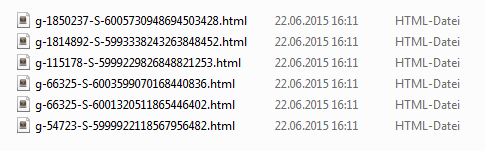
\includegraphics{./images/postdownload.png}
\caption{Heruntergeladene HTML-Seiten von Beitr�gen der Suchanfragen}
\end{figure}

The program has successfully downloaded the 6 documents that the forum has retured for the 10 search queries (figure 18).
This shows that it is possible to register and log in into forums and search for specific (company-specific) keywords for products.